% Created 2018-04-05 Чт 19:06
% Intended LaTeX compiler: pdflatex
\documentclass[presentation]{beamer}
\usepackage[utf8]{inputenc}
\usepackage[T1]{fontenc}
\usepackage{graphicx}
\usepackage{grffile}
\usepackage{longtable}
\usepackage{wrapfig}
\usepackage{rotating}
\usepackage[normalem]{ulem}
\usepackage{amsmath}
\usepackage{textcomp}
\usepackage{amssymb}
\usepackage{capt-of}
\usepackage{hyperref}
\AtBeginSubsection[]{\begin{frame}<beamer>\frametitle{}\tableofcontents[currentsection,currentsubsection]\end{frame}}
\usepackage{pifont}
\usepackage[russian]{babel}
\usepackage[utf8]{inputenc}
\author[]{Кирилл Краснощёков, МГТНИИП}
\usetheme{CambridgeUS}
\usecolortheme{crane}
\date{\today}
\title{Основы работы с git}

\hypersetup{
 pdfauthor={},
 pdftitle={Основы работы с git},
 pdfkeywords={},
 pdfsubject={},
 pdfcreator={Emacs 25.1.1 (Org mode 9.0.5)}, 
 pdflang={Russian}}
\begin{document}

\maketitle
\begin{frame}{Outline}
\tableofcontents
\end{frame}


\section{Введение}
\label{sec:org356d7fa}
\subsection{Что такое системы управления версиями}
\label{sec:orgc1e16f9}
\begin{frame}[label={sec:orgf992b09}]{Что такое система управления версиями}
\begin{columns}
\begin{column}{0.65\columnwidth}
\begin{center}
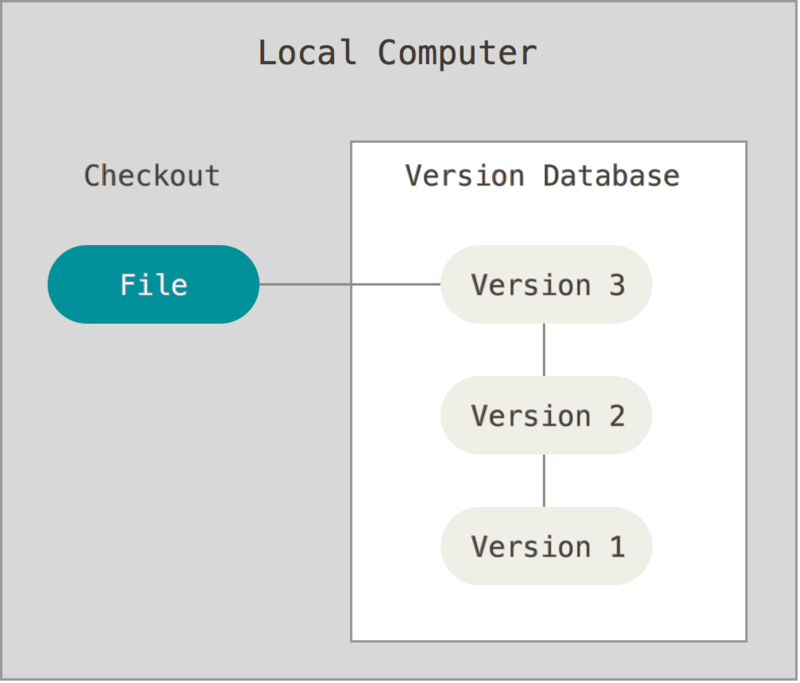
\includegraphics[width=0.8\textwidth]{./01_vcs_00_what.png}
\end{center}
\end{column}

\begin{column}{0.35\columnwidth}
\begin{center}
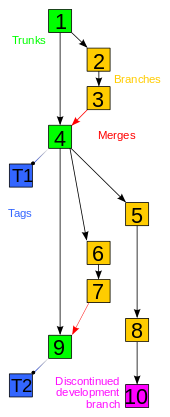
\includegraphics[height=0.8\textheight]{./00_branches_from_wikipedia.png}
\end{center}
\end{column}
\end{columns}
\end{frame}

\begin{frame}[label={sec:orgd70ce89}]{Зачем это нужно}
\begin{itemize}
\item не терять результаты работы
\item работать совместно
\end{itemize}
\end{frame}

\subsection{Термины}
\label{sec:org0ee7043}
\begin{frame}[label={sec:orge58ae94}]{Репозиторий}
Репозиторий = БД изменений в проекте

\begin{center}
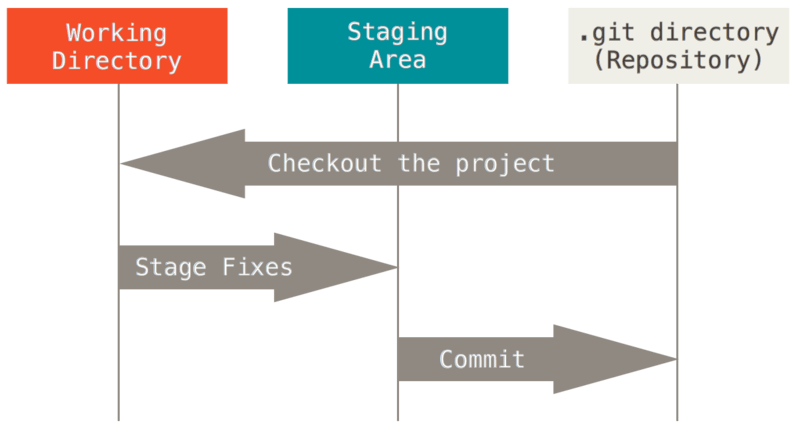
\includegraphics[width=.9\linewidth]{./01_vcs_02_git_directories.png}
\end{center}
\end{frame}

\begin{frame}[label={sec:org3fdff3a}]{Файлы проекта}
\begin{center}
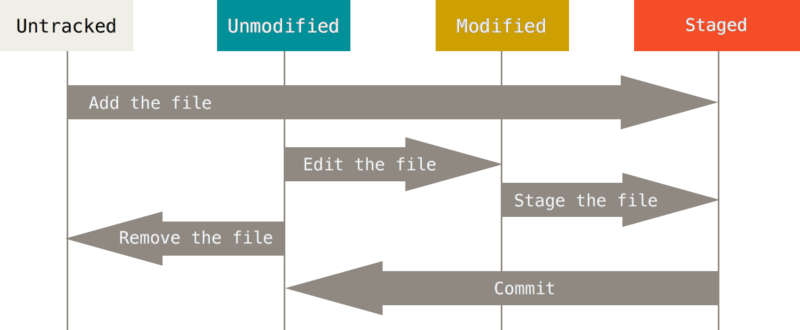
\includegraphics[width=.9\linewidth]{./01_vcs_01_git_file_states.png}
\end{center}
\end{frame}

\section{Как пользоваться}
\label{sec:org92d50fa}
\subsection{Установка, настройка, запуск}
\label{sec:orgc3b3b41}
\begin{frame}[label={sec:org2c43710}]{Установка}
\begin{enumerate}
\item скачать \href{https://git-scm.com/download/win}{последнюю версию}
\item установить (без админских прав)
\end{enumerate}
\end{frame}

\begin{frame}[fragile,label={sec:orgff4b08a}]{Настройка}
 \alert{\texttt{git config}}

\begin{verbatim}
$ git config --global user.name "John Doe"

$ git config --global user.email "john@example.com"
\end{verbatim}
\end{frame}

\begin{frame}[label={sec:org4b113ac}]{Запуск}
\begin{columns}
\begin{column}{0.45\columnwidth}
\begin{center}
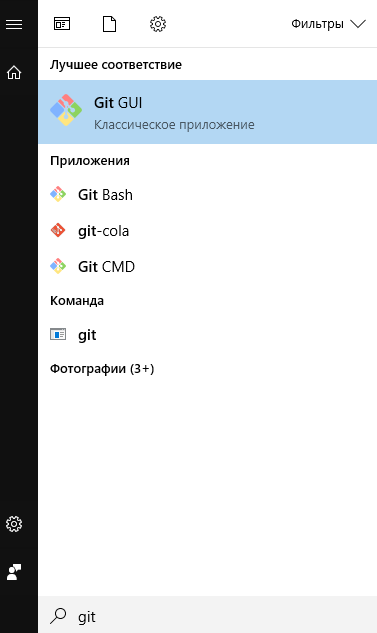
\includegraphics[height=0.8\textheight]{./01_vcs_01_find_git.PNG}
\end{center}
\end{column}
\begin{column}{0.45\columnwidth}
\begin{itemize}
\item git bash
\item git GUI
\end{itemize}
\end{column}
\end{columns}
\end{frame}

\subsection{Как делать резервные копии}
\label{sec:orgc19bc2c}
\begin{frame}[label={sec:org3a9edfd}]{Как делать резервные копии}
\begin{enumerate}
\item создать репозиторий
\item добавить файлы в репозиторий
\item поработать и записать изменения в репозиторий
\end{enumerate}

И повторять шаг 3.
\end{frame}

\begin{frame}[fragile,label={sec:org6ba3b26}]{1. Создать репозиторий}
 \alert{\texttt{git init}}

\begin{verbatim}
$ mkdir project_2

$ cd project_2

$ git init
Initialized empty Git repository in project_2/.git/
\end{verbatim}
\end{frame}

\begin{frame}[fragile,label={sec:org66b5218}]{\ding{43} Осмотреться}
 \alert{\texttt{git status}}

\begin{verbatim}
$ git status
On branch master

Initial commit

nothing to commit (create/copy files 
and use "git add" to track)
\end{verbatim}

\begin{itemize}
\item делайте в любой непонятной ситуации
\end{itemize}
\end{frame}

\begin{frame}[fragile,label={sec:org611fc3b}]{2. Добавить файлы в репозиторий}
 \begin{center}
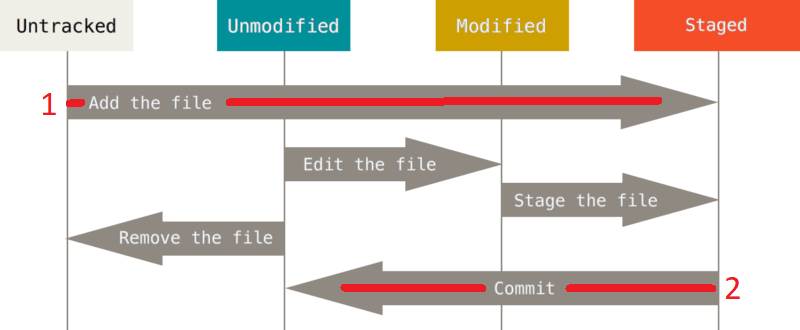
\includegraphics[height=0.5\textheight]{./01_vcs_01_git_file_states_01_add.png}
\end{center}

\begin{enumerate}
\item Поместить файлы в буферную область: \texttt{git add my\_file.txt}
\item Отправить в репозиторий: \texttt{git commit}
\end{enumerate}
\end{frame}

\begin{frame}[fragile,label={sec:org456e2ca}]{- в начале:}
 \begin{columns}
\begin{column}{0.65\columnwidth}
\begin{verbatim}
$ git status
On branch master

Initial commit

Untracked files:
  (use "git add <file>..." to include 
   in what will be committed)

        my_file.txt

nothing added to commit 
but untracked files present 
(use "git add" to track)
\end{verbatim}
\end{column}

\begin{column}{0.35\columnwidth}
\begin{center}
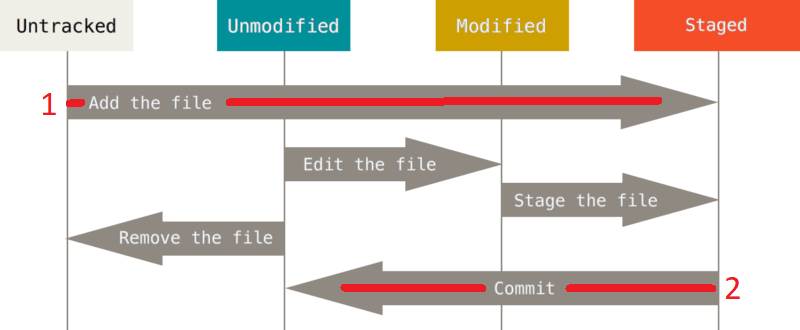
\includegraphics[width=0.98\textwidth]{./01_vcs_01_git_file_states_01_add.png}
\end{center}
\end{column}
\end{columns}
\end{frame}

\begin{frame}[fragile,label={sec:org737c3b7}]{- добавляем файл в буферную область:}
 \alert{\texttt{git add}}

\begin{columns}
\begin{column}{0.65\columnwidth}
\begin{verbatim}
$ git add my_file.txt

$ git status
On branch master

Initial commit

Changes to be committed:
  (use "git rm --cached <file>..." to unstage)

        new file:   my_file.txt
\end{verbatim}
\end{column}

\begin{column}{0.35\columnwidth}
\begin{center}
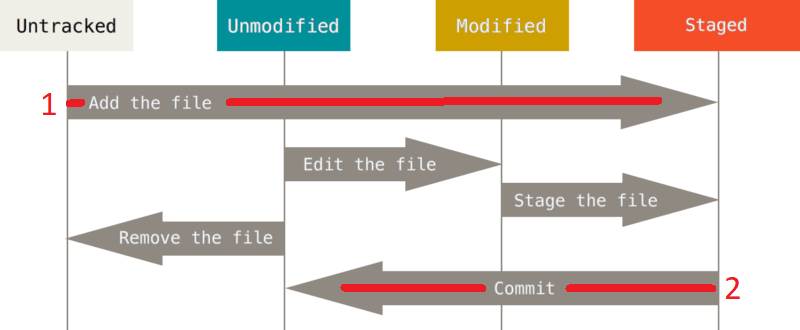
\includegraphics[width=0.98\textwidth]{./01_vcs_01_git_file_states_01_add.png}
\end{center}
\end{column}
\end{columns}
\end{frame}

\begin{frame}[fragile,label={sec:org83efbe3}]{- отправляем изменения в репозиторий:}
 \alert{\texttt{git commit}}

\begin{columns}
\begin{column}{0.65\columnwidth}
\begin{verbatim}
$ git commit -m "Very important change"
[master (root-commit) 2642eb5] Very important change
 1 file changed, 12 insertions(+)
 create mode 100644 my_file.txt

$ git status
On branch master
nothing to commit, working tree clean
\end{verbatim}
\end{column}

\begin{column}{0.35\columnwidth}
\begin{center}
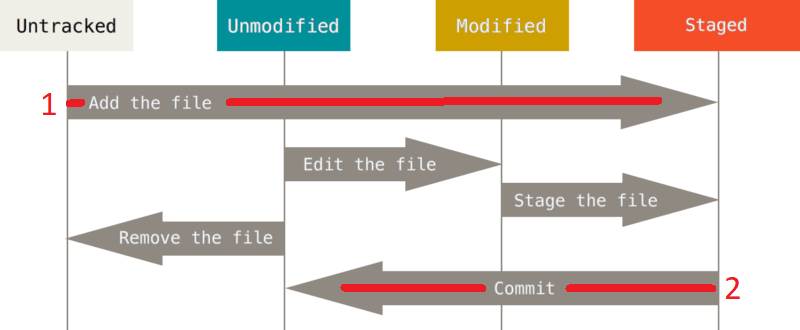
\includegraphics[width=0.98\textwidth]{./01_vcs_01_git_file_states_01_add.png}
\end{center}
\end{column}
\end{columns}
\end{frame}

\begin{frame}[label={sec:org9acb511}]{\ding{43} Комментируйте осмысленно!}
\only<1>{
Так не надо:
 \begin{center}
\includegraphics[width=.9\linewidth]{./xkcd1296_comments.png}
\end{center} 
}

\only<2>{
Так лучше:
\begin{center}
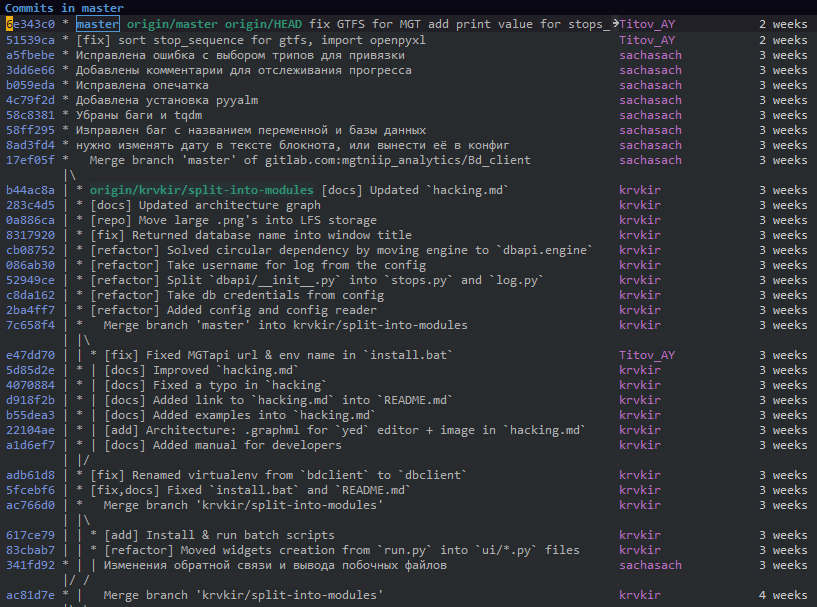
\includegraphics[width=.9\linewidth]{./01_vcs_02_comments.PNG}
\end{center}
}
\end{frame}

\begin{frame}[fragile,label={sec:org3226340}]{3. Записать изменения}
 \begin{center}
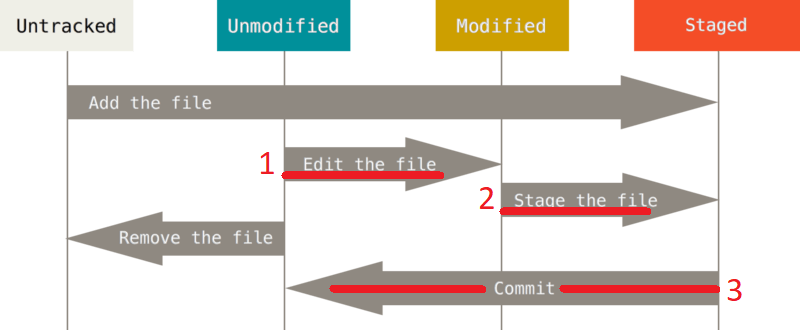
\includegraphics[height=0.5\textheight]{./01_vcs_01_git_file_states_02_change.png}
\end{center}

\begin{enumerate}
\item Поработать
\item Поместить изменённые файлы в буферную область: \texttt{git add my\_file.txt}
\item Отправить в репозиторий: \texttt{git commit}
\end{enumerate}
\end{frame}

\begin{frame}[fragile,label={sec:org36aa1f3}]{\ding{43} Вывести историю}
 \alert{\texttt{git log}}

\begin{verbatim}
$ git log
commit 2642eb5780a454a09bac4ef9113fc029cff27674
Author: krvkir <krvkir@gmail.com>
Date:   Thu Apr 5 12:31:19 2018 +0300

    Very important change
\end{verbatim}
\end{frame}

\subsection{Как несколькоим людям работать над одним проектом}
\label{sec:org9d31fd6}
\begin{frame}[label={sec:org9f0196e}]{Центральный сервер}
\begin{columns}
\begin{column}{0.65\columnwidth}
\begin{center}
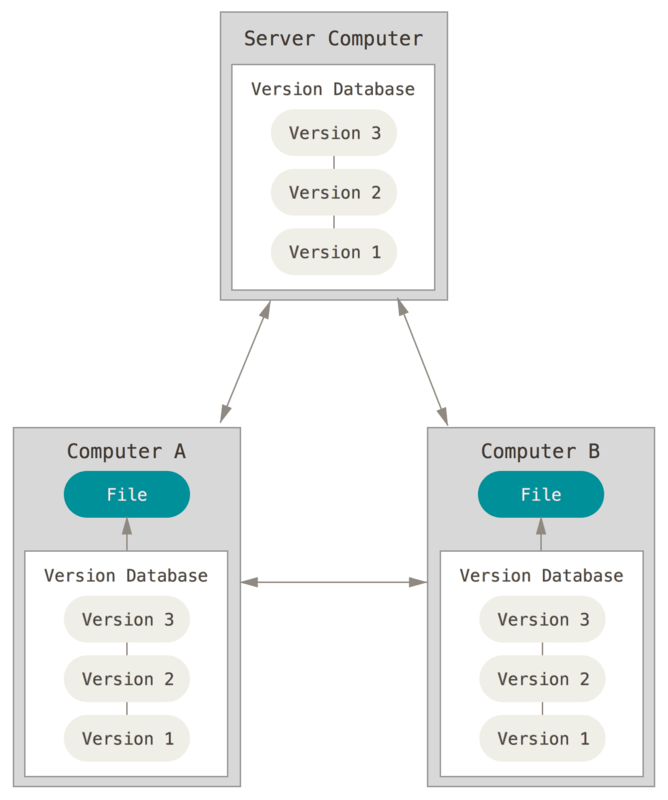
\includegraphics[height=0.8\textheight]{./01_vcs_00_distributed_vcs.png}
\end{center}
\end{column}

\begin{column}{0.35\columnwidth}
\begin{itemize}
\item github.com
\item \alert{gitlab.com}
\item sourceforge.org
\item \ldots{}
\item внутренний сервер
\end{itemize}
\end{column}
\end{columns}
\end{frame}

\begin{frame}[fragile,label={sec:org943c376}]{Как работать с сервером}
 \begin{enumerate}
\item создать репозиторий на сервере
\item клонировать репозиторий с сервера в локальную папку: \texttt{git clone}
\item работать, как обычно
\item отправить изменения на сервер: \texttt{git push}
\end{enumerate}
\end{frame}

\begin{frame}[label={sec:org8a2cecd}]{1. Создать репозиторий}
\begin{center}
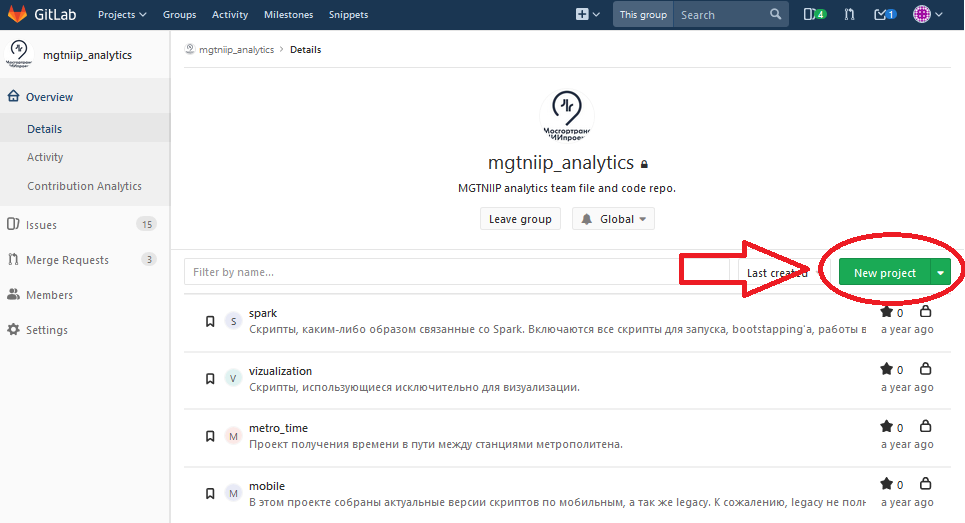
\includegraphics[width=0.8\textwidth]{./01_vcs_03_remote_create_repo.PNG}
\end{center}
\end{frame}

\begin{frame}[label={sec:org6f8333a}]{1. Создать репозиторий}
\begin{center}
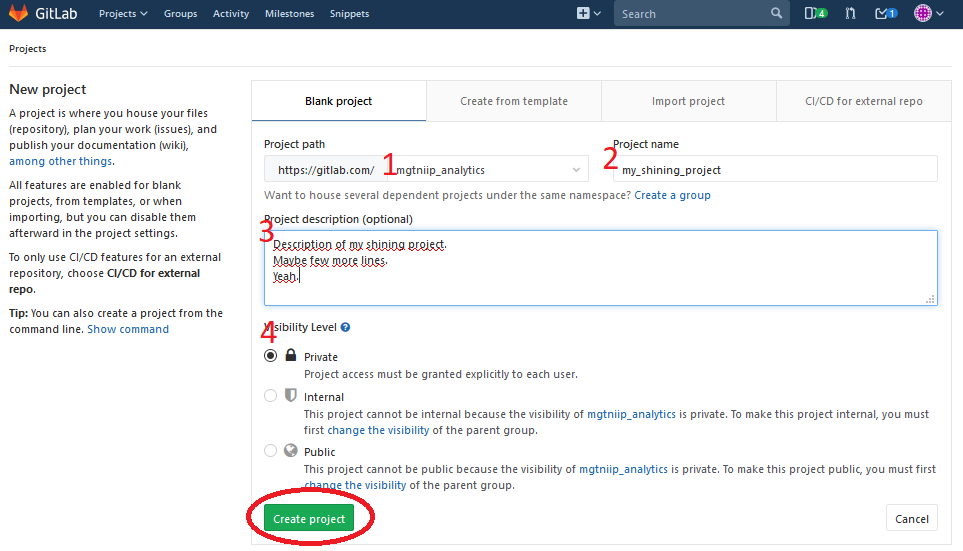
\includegraphics[width=0.8\textwidth]{./01_vcs_03_remote_create_repo_2.PNG}
\end{center}
\end{frame}

\begin{frame}[label={sec:org2f650fb}]{1. Создать репозиторий}
\begin{center}
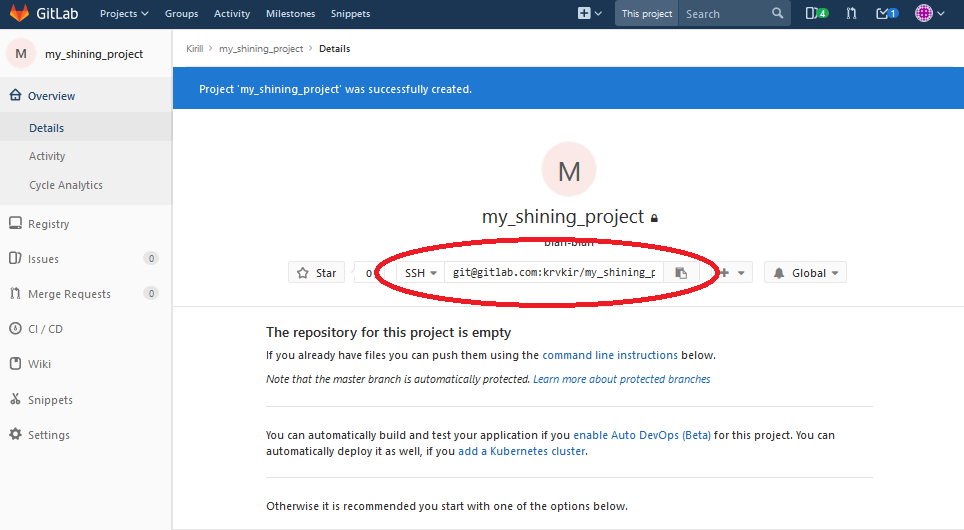
\includegraphics[width=0.8\textwidth]{./01_vcs_03_remote_create_repo_3.PNG}
\end{center}
\end{frame}

\begin{frame}[fragile,label={sec:orgf7212af}]{2. Клонировать репозиторий с сервера}
 \alert{\texttt{git clone}}

\begin{verbatim}
$ git clone https://github.com/krvkir/notes_dev_culture.git                               
Cloning into 'notes_dev_culture'...
remote: Counting objects: 9, done.
remote: Compressing objects: 100% (4/4), done.
remote: Total 9 (delta 2), reused 9 (delta 2), pack-reused 0
Unpacking objects: 100% (9/9), done.

$ cd notes_dev_culture/

$ git status
On branch master
Your branch is up-to-date with 'origin/master'.
nothing to commit, working tree clean
\end{verbatim}
\end{frame}

\begin{frame}[fragile,label={sec:orga45b419}]{\ding{43} Список серверов}
 \alert{\texttt{git remote}}

\begin{verbatim}
$ git remote
origin

$ git remote -v
origin  git@github.com:krvkir/notes_dev_culture.git (fetch)
origin  git@github.com:krvkir/notes_dev_culture.git (push)
\end{verbatim}
\end{frame}

\begin{frame}[fragile,label={sec:org537b4ee}]{3. Работать, как обычно}
 \begin{center}
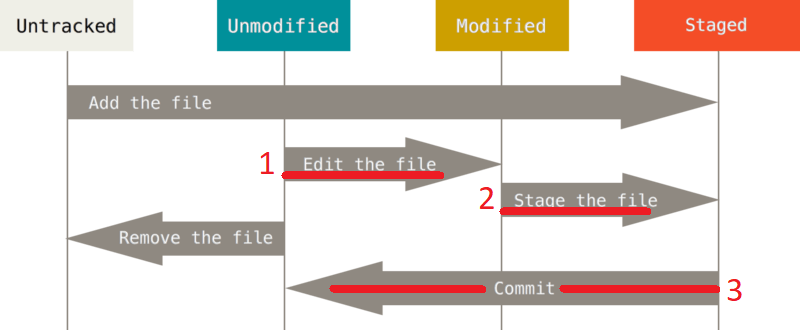
\includegraphics[height=0.5\textheight]{./01_vcs_01_git_file_states_02_change.png}
\end{center}

\begin{enumerate}
\item Поработать
\item \texttt{git add}
\item \texttt{git commit}
\end{enumerate}
\end{frame}

\begin{frame}[fragile,label={sec:org80552f7}]{4. Отправить изменения на сервер}
 \alert{\texttt{git push}}

\begin{verbatim}
git push origin master
\end{verbatim}

\begin{itemize}
\item ввести логин и пароль от \alert{сервера}
\end{itemize}
\end{frame}

\subsection{Как взять обновления с сервера}
\label{sec:orgefc9251}
\begin{frame}[fragile,label={sec:org1f0d292}]{Как взять обновления с сервера}
 \begin{enumerate}
\item Скопировать репозиторий с сервера: \texttt{git clone}
\item Обновить: \texttt{git pull}
\end{enumerate}

\begin{verbatim}
$ git pull origin master
\end{verbatim}
\end{frame}

\begin{frame}[label={sec:orgdefbc5e}]{Материалы}
\begin{itemize}
\item \href{https://git-scm.com/book/ru/v2}{Pro Git} (книга)
\item \href{http://gitvisual.com}{Git Visual} (интерактивная обучалка)
\end{itemize}
\end{frame}
\end{document}
